\section{What was your first boss like?}
I'll name my job at Provident Bookstore as my first formal job.
While I in high school I began working in the Lancaster store on E King Street.
My job was a behind the scenes job in what was called the traffic department.
I unpacked and counted the orders of items that came into the store.
I remember often working by myself in the basement room.
I do not remember who my boss was for that job.

When Provident Store moved to the large Park City mall west of town I applied for and got a job working on the floor in that store.
I remember working the cash register, helping people find books and selling Bibles.
When we sold a certain number of Bibles we received one free.
Working at Provident Bookstore evenings and Saturdays helped me pay my way through the four years at Millersville College.
My boss during this job was Nevin Horst.
\begin{figure}
\centering
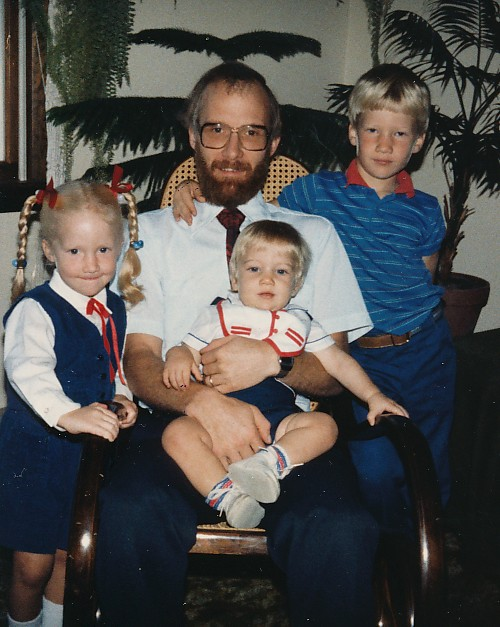
\includegraphics[width=0.4\textwidth]{finding_my_way/3.jpg}
\caption{
Nevin Horst
}
\end{figure}

He was not a demanding supervisor and had a low key sense of humor.
I remember him as a kind person to be around.
I still remember receiving a phone call from him that left me laughing, giddy with silliness.
The managers of the stores in the Park City Mall were invited to enter their employees into a drawing for a one day trip to the Bahama Islands.
I was not aware that he had entered all of the bookstore employee's names.
My name was one of those drawn as a winner.

Some weeks later it all felt surreal to arrive at the airport early before sunrise and board the plane for the Bahama Islands.
Since this was a trip for two I invited my friend Linda to travel with me.
I remember Linda and I were some of the few people who took juice or soda rather than alcoholic drinks during the flight.
I remember visiting a market, walking the streets, and wading in the water so blue and clear that I could see my toes in the sand.
Then as the day turned toward sunset we got back on the plane and returned to world of classes, studies, and work at Provident Store.

Nevin has died but I met his widow Blanche in recent years and she greeted me as someone she knew and appreciated.
They were both good at letting people know they are of value.

From Abby - Wow Mom! I can't believe I didn't know about you winning a day trip to the Bahamas! What an incredible experience.
Were you still dressing conservatively at that point?
From Tim - I also had never heard the Bahamas story.
I love these descriptions:
"I still remember receiving a phone call from him that left me laughing, giddy with silliness.
"
"They were both good at letting people know they are of value.
"
It's interesting that these are both personality traits that I learned to value from you and Dad and strive to live up to in my own life.

From Mom - I actually still had long hair and wore it up in a bubble rather than a bun.
I do not remember if I wore a covering that day or not.
Given it was still my daily practice I probably did.
Attached is my college graduation photo.
I was a college student at Millersville College when I made this trip to the Bahamas.






